\documentclass[11pt, a4paper]{article}




\usepackage[utf8]{inputenc}		% Zeichen in UTF-8 speichern (?)
\usepackage[T1]{fontenc}		% Sonderzeichen richtig darstellen
\usepackage[british]{babel}		% versch. Sonderzeichen, Silbentrennung, Gliederung
\usepackage[margin=25mm, top=38mm, bottom=20mm, headheight=40pt]{geometry}
\usepackage{fancyhdr}			% Kopf- und Fußnoten
\usepackage{multicol}			% mehrere Spalten
\usepackage{lastpage}			% Seite x von y
\usepackage{tabularx}    		% Tables of specified width
\usepackage{graphicx}			% Einstellmöglichkeiten für Bilder
\usepackage{caption}			% Einstellmöglichkeiten Tabellen- und Bildunterschriften, captionof
\usepackage{array}
\usepackage{booktabs}
\usepackage{siunitx}			% SI-Einheiten
\usepackage{mathtools}			% macht die Matheumgebung, Weiterentwicklung von amsmath
\usepackage{amssymb}			% Erweiterung des Zeichensatzes, beinhaltet amsfonts
\usepackage{verbatim}			% macht die "comment-Umgebung"
\usepackage[hidelinks]{hyperref}
\usepackage{setspace}





%\addto{\captionsbritish}{
%\renewcommand{\figurename}{Fig.}
%\renewcommand{\tablename}{Tab.}
%}


\setlength{\parindent}{0pt}

\setlength{\columnsep}{8mm}

\clubpenalty10000
\widowpenalty10000
\displaywidowpenalty = 10000


\pagestyle{fancy}
\fancyhf{}
\lhead{something}
\rhead{Page \thepage\ of \pageref{LastPage}}


% new column types for tabularx
\newcolumntype{Y}{>{\raggedright\arraybackslash}X} % X column left aligned
\newcolumntype{W}{>{\raggedleft\arraybackslash}X}  % X column right aligned
\newcolumntype{Z}{>{\centering\arraybackslash}X}   % X column centered


\newenvironment{Figure}
  {\par\medskip\noindent\minipage{\linewidth}}
  {\endminipage\par\medskip}
\renewcommand{\arraystretch}{1.2}


\sisetup{per-mode = symbol}











\begin{document}

\begin{titlepage}
\centering
{somebody make a fancy title page}
\end{titlepage}





\tableofcontents





\newpage
\section{Introduction}

somebody write an introduction \\

bl.a. mention
\begin{itemize}
\item where we get the forward model from and what it does (this will not be explained in the following section)
\item that we need the forward model to do the inverse model (which was the actual task)
\item emphasize that the ref data is from numerical weather predictions and not necessarily correct
\end{itemize}






\newpage
\section{Validation of the Forward Model}

The forward model computes from a set of oceanic and atmospheric parameters the brightness temperatures expected to be measured by a satellite radiometer. The input parameters are listed in Table \ref{tab:input_parameters}, and the output parameters include values for both horizontal and vertical polarization at \SI{6.93}{GHz}, \SI{10.65}{GHz}, \SI{18.70}{GHz}, \SI{23.80}{GHz}, and \SI{36.50}{GHz}.

\begin{table}[h!]
\centering
\begin{tabular}{@{}p{4cm} p{1.8cm}p{2.8cm}p{1.8cm}p{1.8cm}@{}}
%\toprule
\tabularnewline
& \multicolumn{2}{c}{Forward Model} & \multicolumn{2}{c}{Reference Data}
\tabularnewline
\cmidrule(r{1em}){2-3} \cmidrule(l{1em}){4-5}
& Abbrev. & Unit & Abbrev. & Unit
\tabularnewline
\midrule
Ice concentration	& C\_is	& fraction		& ci	& fraction	\\
MY-fraction		& F\_MY	& fraction		& 	& 		\\
Ice temperature		& T\_is	& \SI{}{K}	& skt	& \SI{}{K}	\\
Water vapour		& V	& \SI{}{mm} (columnar)	& tcwv	& \SI{}{kg/m^2}	\\
Cloud liquid water	& L	& \SI{}{mm} (columnar)	& tclw	& \SI{}{kg/m^2}	\\
Wind speed		& W	& \SI{}{m/s}		& ws	& m/s		\\
Sea surface temperature	& T\_ow	& \SI{}{K}	& sst	& \SI{}{K}	\\
\midrule
\end{tabular}
\caption{Atmospheric and oceanic parameters entered into the forward model}
\label{tab:input_parameters}
\end{table}

This forward model was validated by comparing its results to reference data from ESA's ``Sea Ice Climate Change Initiative''.



\subsection{Description of the Reference Data}
\label{sec:RefDat}

The reference data consists of brightness temperatures at the relevant polarizations and frequencies as measured by the AMSR2 radiometer onboard the GCOM-W1 satellite. %for a range of geocoded locations at a given time.
The measured data is paired with validated sea ice concentrations and numerical weather predictions for the atmospheric and oceanic parameters at the same geocoded locations at near simultaneous time. There are two different data sets: one with an ice concentration of 0, the other one with an ice concentration of 1. The data points of each set cover the entire year 2014. The dataset with the no ice condition covers latitudes between 5 and 73 degrees, and the dataset with an ice concentration of 1 covers latitudes betwwen 78.5 and 87.5 degrees. 
\newline

When using this reference data package to validate the forward model, several points have to be taken into account: Firstly, the forward model was developed for the AMSR-E instrument. By using the atmospheric and oceanic parameters as input in the forward model in order to compare the output with the AMSR2 measured brightness temperatures, we assume that any calibration differences between AMSR-E and AMSR2 are negligible. % Advanced Microwave Scanning Radiometer (AMSR) 
%The AMSR-E instrument on the NASA satellite EOS Aqua was operational between May 4, 2002 and October 4, 2011, and the AMSR2 instrument mounted on the JAXA satellite GCOM-W1, has been in operation since May 18, 2012. 
\newline

Secondly, the reference data does not contain information about the multi-year ice fraction needed as input in the forward model. %The multi-year ice fraction cannot be found in the reference data and should therefore be determined by other means. The reference data is divided into two parts, one contains only datapoints from areas of open water for which the ice concentration is zero in which case
For the data set with an ice concentration of 0, the MY fraction is irrelevant. It is therefore possible to validate the forward model for the open water datapoints. For the data set with an ice concentration of 1, %The other part of the reference data contain datapoints from areas of high ice concentration for which the MY fraction is unknown. 
a multi-year ice concentration of 0.5 was found to produce reasonable outputs of the forward model. This dataset can therefore be used as a coherency check, but not to validate the model.
%We will still attempt to test the forward model for the high ice concentration areas by making an estimate of the MY fraction through a process of trial and error. The idea is to select a location where we have prior information about the MY fraction(...).
\newline

Thirdly, the wind speed is given in the %NWP
reference data as a u-component, v-component, and as a composite of the two. %(comment/question: where u and v denote zonal and meridional directions respectively?)
To simplify the validation procedure, we used the composite value for the wind speed as the input in the forward model. %(Argumentation!?) (-backscatter as a result of wind speed direction (upwind, downwind, crosswind) sensitive to azimuth angle \cite{Elachi})
\newline

%In order to use the reference data in the forward model it was necesarry to perform unit conversions for 
The parameters ``water vapour'' and ``cloud liquid water'', which are given in the columnar units of $\SI{}{kg/m^2}$ in the reference data, were converted to $\SI{}{mm}$, indicating the height of water vapor or cloud liquid water if condensed uniformly across the column. $\SI{1}{kg/m^2}$ corresponds to $\SI{1}{mm}$ \cite{remss}.


\subsection{Validation Procedure}

For the data set with an ice concentration of 0, the atmospheric and oceanic parameters were entered into the forward model, and the difference of the modelled brightness temperatures with respect to the reference data was recorded. The reference file has 6988 data points, all of which were used. For the data set with an ice concentration of 1, the atmospheric and oceanic parameters were entered together with a guessed value for the multi-year ice fraction. This value was chosen to be constant for all datapoints to simplify the validation process.


\subsection{Validation Results}
\label{sec:ForValRes}

The discrepancies for the no ice condition are shown in Figure \ref{fig:for0}, and those for the ice condition are shown in Figure \ref{fig:for1}. Later in this report, the inverse model will be used to develop an estimation of the impact a certain discrepancy in brightness temperature has on the modelled atmospheric and oceanic parameters.

\begin{figure}[h]
   \centering
   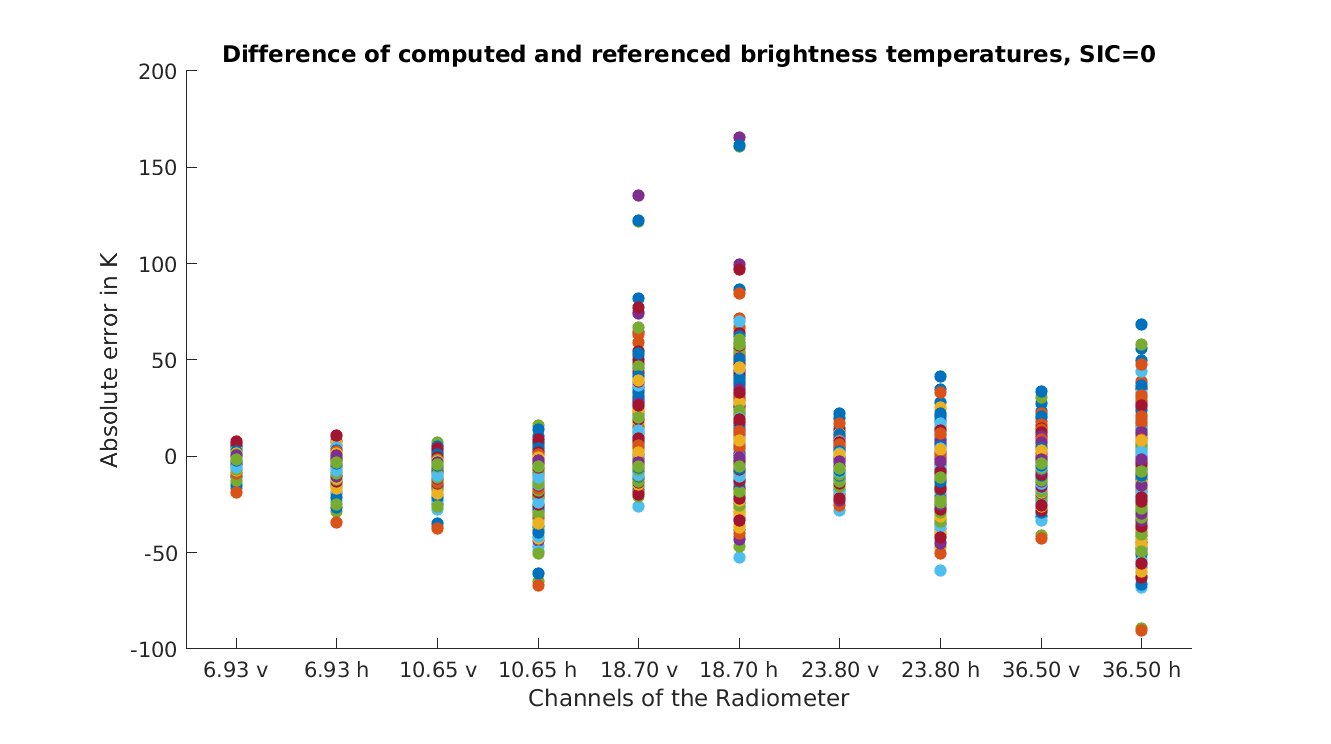
\includegraphics[width=0.9\textwidth]{ValidationForward_SIC0.eps}
   \caption{Modelled brigthness temperatures compared to the no ice dataset}
   \label{fig:for0}
\end{figure}

\begin{figure}[h]
   \centering
   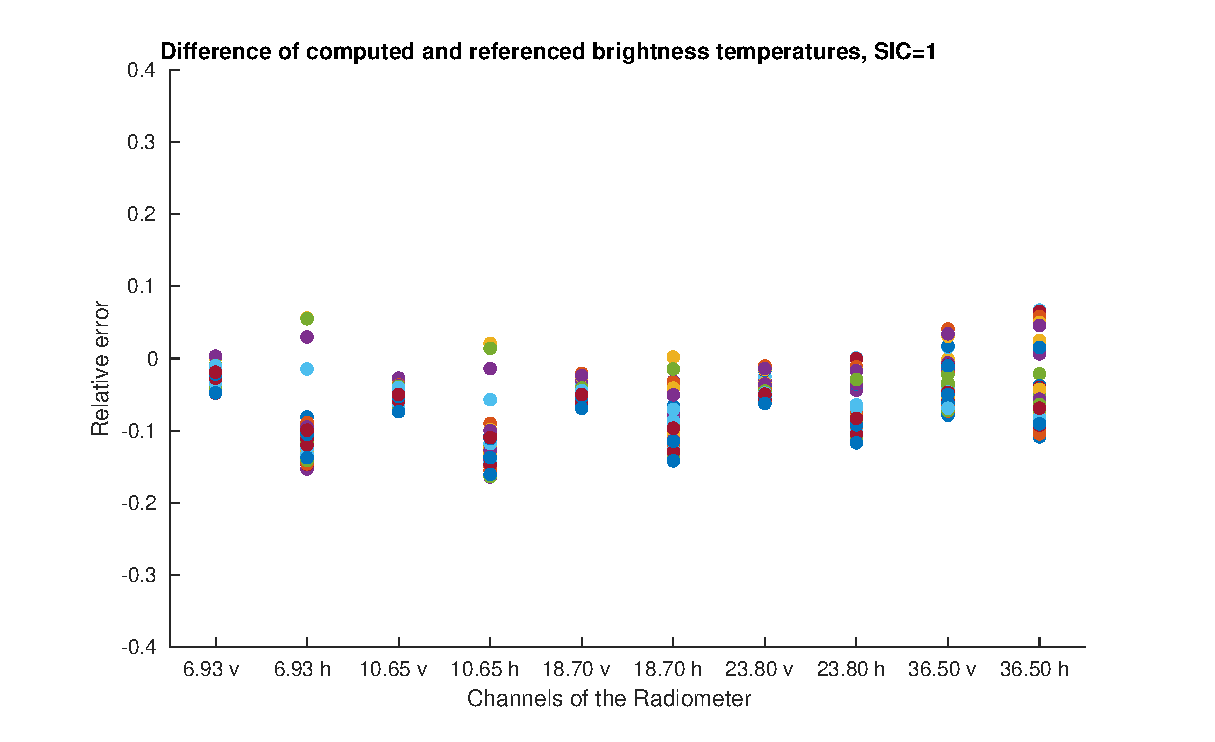
\includegraphics[width=0.9\textwidth]{ValidationForward_SIC1.eps}
   \caption{Modelled brigthness temperatures compared to the dataset with an ice concentration of 1}
   \label{fig:for1}
\end{figure}

\begin{figure}[h!]
   \centering
   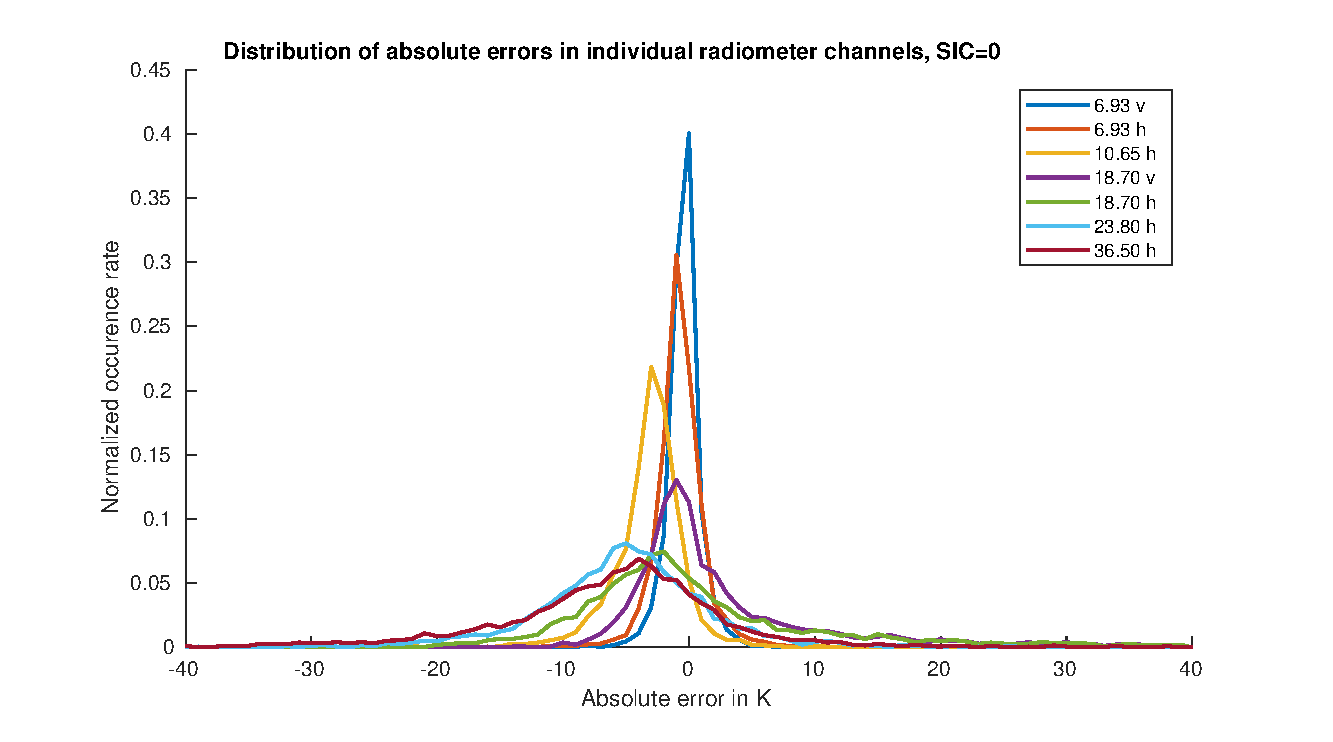
\includegraphics[width=0.9\textwidth]{ValidationForward_SIC0_errordist.eps}
   \caption{Distribution of the errors of the modelled brightness temperatures compared to the no ice dataset; only some channels are shown}
   \label{fig:for1dist}
\end{figure}

For the no ice condition, the discrepancies in channels 10.65 h, 18.70 v and h, 23.80 h, and 36.50 h exceed \(\pm\)\SI{50}{K}. A histogram of the error distribution of these channels was plotted, see \mbox{Figure \ref{fig:for1dist}}. The modelled brightness temperatures appear to have an offset of approx. \SI{-8}{K}, with a tendency to a higher offset for the higher frequencies. For the channels 10.65 h and 18.70 v, \SI{90}{\percent} of the errors lie within \(\pm\)\SI{10}{K} off the offset (mean error) of that channel. For the channels 18.70 v and 23.80 h, \SI{90}{\percent} of the errors lie within \(\pm\)\SI{20}{K} off the offset, and for the channel \mbox{36.50 h}, \SI{90}{\percent} of the errors lie within \(\pm\)\SI{30}{K} off the offset.
\newline

The absolute error of the modelled data compared to the dataset with an ice concentration of 1 appears smaller than for the comparison to the dataset with the no ice condition. However, the minimization of this error was used as the criterion to find the best guess for the multi-year ice concentration. It is therefore not feasible to use this set of errors as a means of describing the accuracy of the forward model.






\clearpage
%\newpage
\section{Development of the Inverse Model}

To compute the oceanic and atmospheric parameters from the set of brightness temperatures measured by the satellite radiometer, an inverse model was developed using estimation theory. The inverse model essentially employs the forward model to compute an estimate of the brightness temperatures from an estimate of the geophysical parameters, then compares the estimated brightness temperatures to the measured brightness temperatures, and finally improves the estimate for the geophysical parameters based on the result of the comparison (see figure \ref{fig:block} for a graphical representation). Once the estimated brightness temperatures come close enough to the measured ones, the geophysical parameters last inputted are considered a good estimate and delivered as the result of the inverse modelling. This is explained in more detail in the next subsection.
\newline

The inverse model was then validated by comparing it to the forward model. It was not compared to any external data source.


\subsection{Algorithm of the Inverse Model}

The input of the inverse model function is a 10 element vector \(T_\text{B,m}\) containing the brightness temperatures measured for each of the radiometer channels.
\newline

\begin{figure}[h]
   \centering
   \includegraphics[width=0.6\textwidth]{blockdiagramm.pdf}
   \caption{Blockdiagramm of the inverse model function}
   \label{fig:block}
\end{figure}


The inverse model enters a 7 element vector \(p\) containing estimates of the geophysical parameters listed in table \ref{tab:input_parameters} into the forward model and retrieves a 10 element vector \(T_\text{B,e}\) containing estimated brightness temperatures for each channel. In the first iteration, \(p\) is a generic guess, which is hard coded into the inverse model function. The estimated brightness temperatures \(T_\text{B,e}\) are then compared to the measured brightness temperatures \(T_\text{B,m}\).
\newline

If the estimated and the measured brightness temperatures do not agree within a range of \(\varepsilon\), a vector \(p_{n+1}\) for the (n+1)\textsuperscript{th} iteration is computed from the vector \(p_n\) of the current iteration as follows:

\begin{equation*}
p_{n+1} =
p_n   +   \Big(S_p^{-1} + M_n^T S_e^{-1} M_n \Big)^{-1}   \cdot   \Big(M_n^T S_e^{-1} (T_\text{B,m} - T_\text{B,e,n}) + S_p^{-1} (p_0 - p_n) \Big)
\end{equation*}

\ \\
Herein, \(S_p\) is the 7 by 7 covariance matrix of the geophysical parameters indicating the uncertainty attached to the start guess. Small values on the diagonal of this matrix correspond to a high confidence in the start guess and cause \(p_{n+1}\) to be close to \(p_0\). \(S_e\) is the 10 by 10 covariance matrix of the brightness temperatures measured by the radiometer. Small values on the diagonal of this matrix correspond to a high confidence into the accuracy of the radiometer, and much weight is assigned to the difference between the estimated and measured brightness temperatures, accordingly.
\newline

\(M_n\) is a 7 by 10 matrix, and it contains the partial derivatives of the brightness temperatures with respect to the geophysical parameters. This matrix is computed for every iteration. To find the element in the i\textsuperscript{th} line and j\textsuperscript{th} column of \(M\), the i\textsuperscript{th} geophysical parameter is perturbed slightly, the forward model is called for the altered vector p, and the resulting perturbation of the brightness temperature in the j\textsuperscript{th} channel is recorded. The partial derivative is then obtained by dividing the brightness temperature perturbation by the perturbation of the geophysical parameter. Large values in \(M\) correspond to a high sensitivity of the radiometer to changes in the geophysical parameters.
\newline

The partial derivatives are only valid for those values of \(p\) at which they were computed - i.e. those of the past iteration. The inverse model extrapolates these derivatives to find \(p_{n+1}\) for the next iteration. If the relations of the geophysical parameters and the brightness temperatures were entirely linear, this extrapolation would be entirely accurate and only one iteration would be needed to find the suitable vector \(p\). The less linear the system is, the less accurate is the extrapolation, and the more iterations are needed.
\newline

If the estimated and the measured brightness temperatures do agree within a range of \(\varepsilon\), the current vector p is outputted as a sufficiently accurate estimation of the geophysical parameters.


\subsection{Choice of Model Parameters}

Suitable values for the start guess of the atmospheric and oceanic parameters (\(p_0\)) and for the covariance matrix \(S_p\) were found by computing the mean and variance of the individual parameters from the reference data sets. As the data sets cover all seasons and almost the entire globe (see section \ref{sec:RefDat}), we believe this reference to be a broad enough base for computing a generic mean and variance. The values for both are listed below; the elements being in the order wind speed, water vapour, liquid water, sea surface temperature, ice temperature, ice concentration, multiyear ice fraction. The units correspond to those given in \mbox{table \ref{tab:input_parameters}}.

\begin{equation*}
p_0 =
\begin{pmatrix}
   6.1327 & 7.7035 & 0.0295 & 273.5503 & 265.0088 & 0.5000 & 0.5000
\end{pmatrix}
\end{equation*}

\begin{equation*}
S_p =
\begin{pmatrix}
   9.2865 & 0 & 0 & 0 & 0 & 0 & 0 \\
   0 & 62.1415 & 0 & 0 & 0 & 0 & 0 \\
   0 & 0 & 0.0056 & 0 & 0 & 0 & 0 \\
   0 & 0 & 0 & 22.5386 & 0 & 0 & 0 \\
   0 & 0 & 0 & 0 & 98.6461 & 0 & 0 \\
   0 & 0 & 0 & 0 & 0 & 1 & 0 \\
   0 & 0 & 0 & 0 & 0 & 0 & 1
\end{pmatrix}
\end{equation*}

\ \\
For each of the radiometer channels, an uncertainty of \SI{0.4}{K} was assumed. This leads to \SI{0.16}{K^2} for each element of the diagonal of \(S_e\).


\subsection{Validation Procedure}

The inverse model is intended to be an inversion of the forward model. This means that in comparison to any reference, the inverse model can at most be as accurate as the forward model. The inverse model was therefore validated by comparison to the forward model: brightness temperatures for a given set of geophysical parameters were computed by the forward model, these brightness temperatures were entered into the inverse model to compute an estimate of the geophysical parameters (\(p_e\)), and the estimate was then compared to the original set of geophysical parameters (\(p_o\)).
\newline

The reference data sets used to validate the forward model were used as a generic source of geophysical parameters to be inputted into the forward model. They were not used as a reference to compare modelled results to!
\newline

We chose to describe the error of the inverse model as follows:

\begin{equation*}
e = \frac{p_\text{e} - p_\text{o}}{\sigma}
\end{equation*}

By normalizing to the standard deviation \(\sigma\), the dependancy of the individual parameters on units is removed. This normalization can be interpreted as adjusting the unit of each parameter such that the original distribution has a standard deviation of 1. For example, an error of 0.5 would then mean a deviation of the estimated parameter by 0.5 times the standard deviation of that parameter when observed on the whole globe and over the course of one year.
\newline

The normalization to the standard deviation introduces a systematic error source into the validation of the inverse model, because the same data sets that were used to compute the standard deviation were already used for the optimization of this model. The independence of development and validation is thus violated. However, we consider the data base to be broad enough to neglect this error.

\begin{comment}
- compute new std dev: expect that it becomes larger = the loop creates additional "inconfidence"
or talk about the distribution of the error? --> histogram with seven lines?
\end{comment}


\subsection{Validation Results}

The error produced by the inverse model was plotted into separate diagrams for the two ice concentrations, see figures \ref{fig:inv0} and \ref{fig:inv1}. Unfortunately, the accuracy appears to depend on the type of input. To investigate the exact reason for the increased uncertainty for the no ice condition, one could divide the datasets into smaller groups of common latitude, season, or magnitude of input parameters, and then record the error distribution for each subset. However, this has not been done so far, and more reference data might be necessary.

\begin{figure}[h]
   \centering
   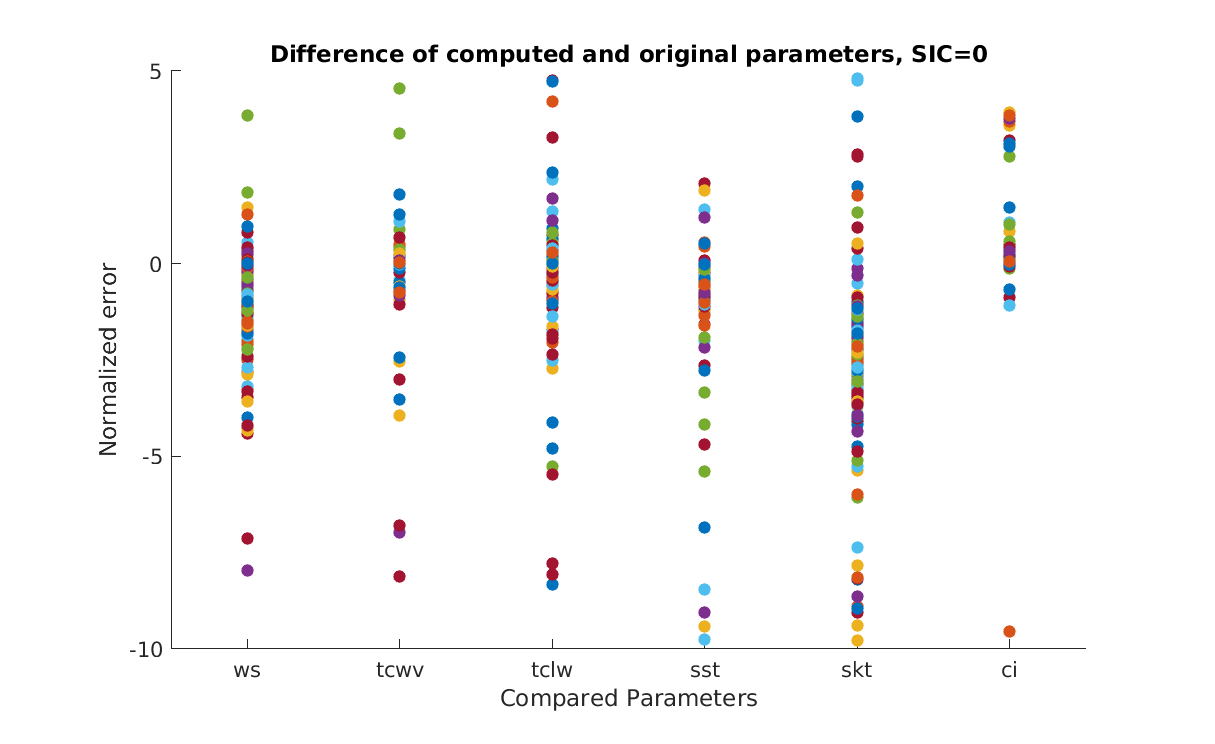
\includegraphics[width=0.9\textwidth]{ValidationInverse_SIC0.eps}
   \caption{Error of the computed geophysical parameters for input data from equatorial and mid-latitude regions}
   \label{fig:inv0}
\end{figure}

\begin{figure}[h]
   \centering
   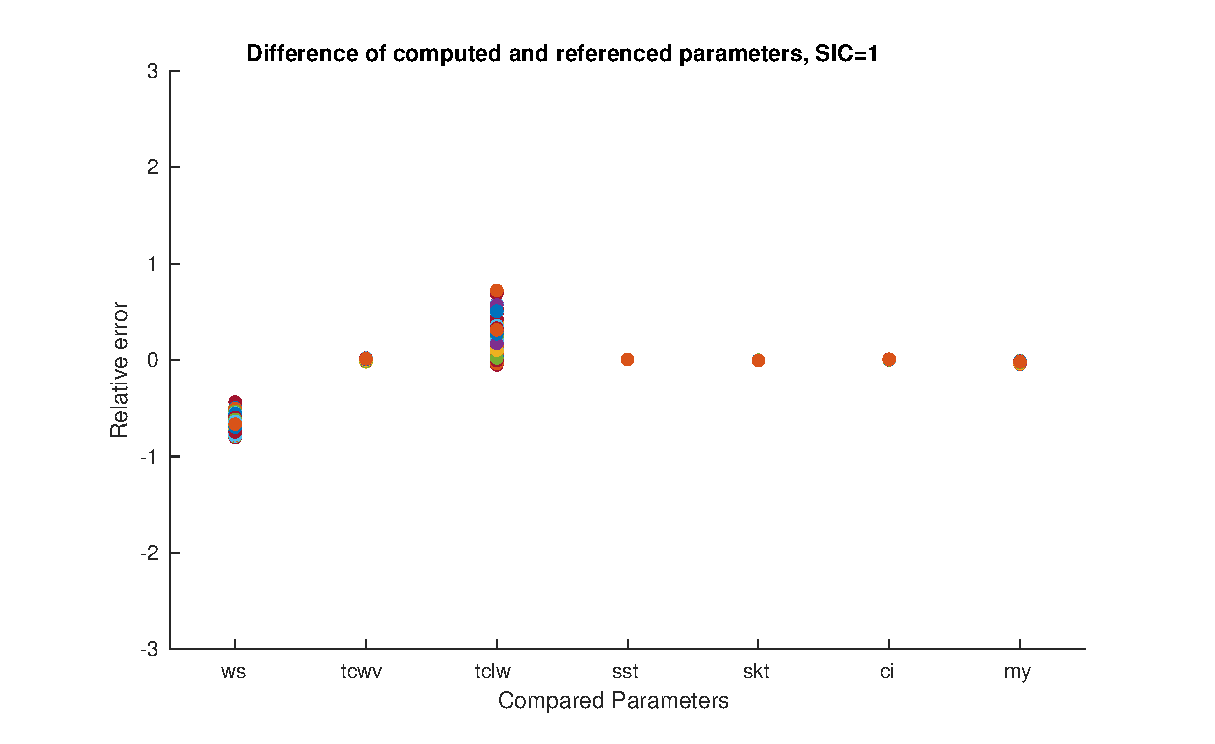
\includegraphics[width=0.9\textwidth]{ValidationInverse_SIC1.eps}
   \caption{Error of the computed geophysical parameters for input data from polar regions}
   \label{fig:inv1}
\end{figure}

\ \\
For input data from the no ice condition, some outliers are not being displayed in figure \ref{fig:inv0} in order to keep the scale readable where most of the errors lie. This affects less than \SI{1}{\percent} of the data points in this set. To gain a better understanding of the distribution of the error, which appears particularly broad in this figure, histograms of the error distributions are shown in figure \mbox{\ref{fig:inv1dist}} for the no ice dataset.

\begin{figure}[h]
   \centering
   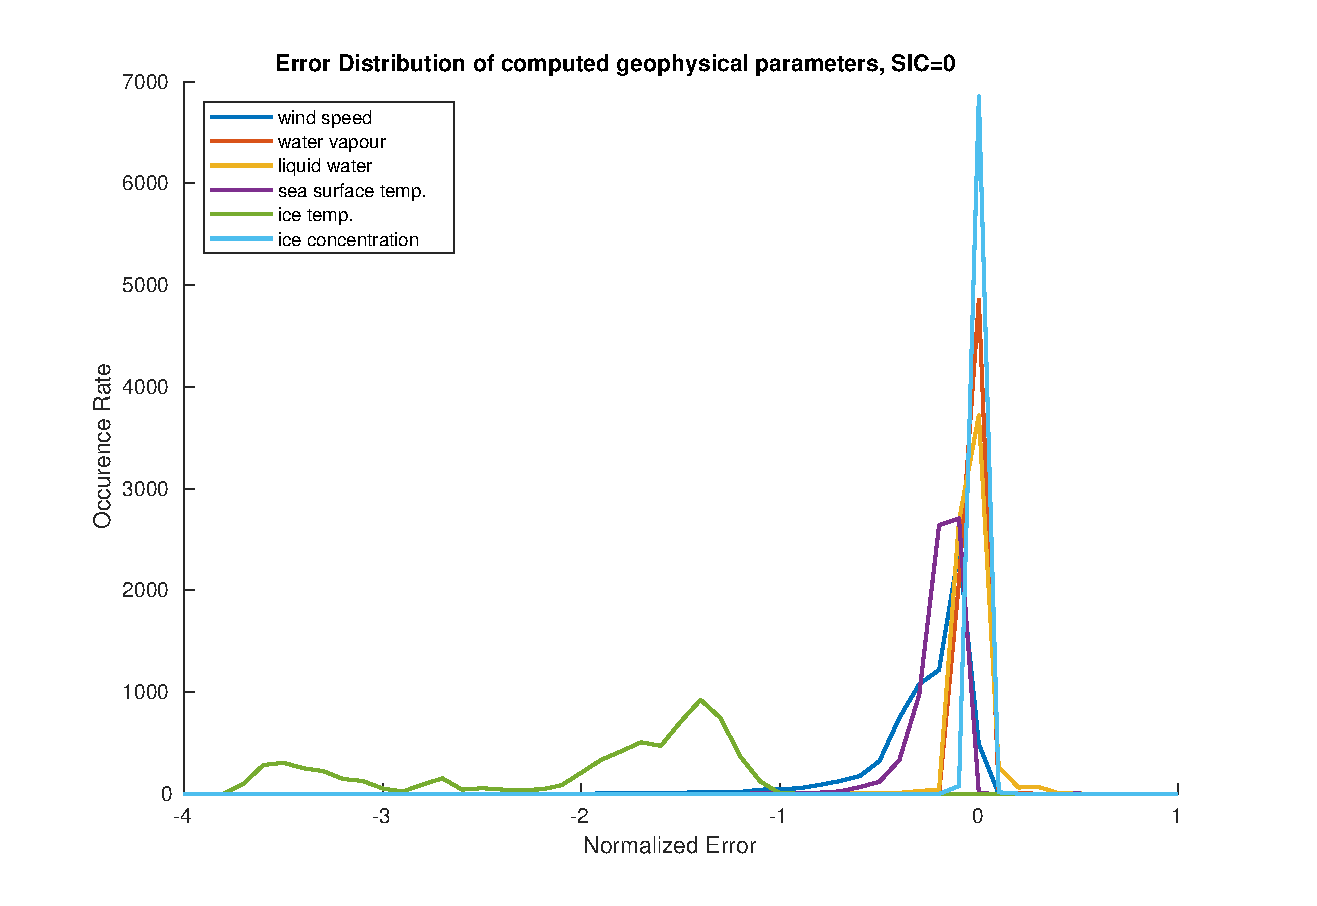
\includegraphics[width=0.9\textwidth]{ValidationInverse_SIC0_errordist.eps}
   \caption{Distribution of the error of the computed geophysical parameters for input data from equatorial and mid-latitude regions; the data set contains 6988 data points}
   \label{fig:inv1dist}
\end{figure}








\clearpage
\section{Application of the Inverse Model}

\subsection{Summary: Uncertainties}

In section \ref{sec:ForValRes}, the discrepancy between the forward model and the reference data was given in terms of brightness temperatures. To gain a better understanding of the significance of a certain error in brightness temperature, the inverse model was applied to compute the error in the geophysical parameters, which corresponds to adding the root mean square error \(\Delta \ T_\text{B}\) of the brightness temperatures given in figure \ref{fig:for0} to the mean value of the brightness temperatures given in the relevant reference data set.

\begin{align*}
& T_\text{B, mean} =  \\
& [ 165.350 \ 84.003 \ 173.818 \ 91.790 \ 195.326 \ 120.459 \ 216.186 \ 159.302 \ 218.686 \ 157.268 ] \\ \\
& \Delta \ T_\text{B} =  \\
& [ 2.378 \ 3.907 \ 5.462 \ 6.899 \ 9.937 \ 12.585 \ 6.556 \ 11.396 \ 6.194 \ 13.484 ] \\ \\
& T_\text{B, mean + rms error} = \\
& [ 167.728 \ 87.910 \ 179.280 \ 98.689 \ 205.263 \ 133.044 \ 222.742 \ 170.698 \ 224.880 \ 170.752]
\end{align*}

\ \\
The atmospheric and oceanic parameters computed for the two brightness temperature vectors above are shown in table \ref{tab:perror}.

\begin{table}[h!]
\centering
\begin{tabular}{@{} l l l l l l l @{}} \tabularnewline
& ws & tcwv & tclw & sst & skt & ci \\
& [\SI{}{m/s}] & [\SI{}{kg\per\square\meter}] & [\SI{}{kg\per\square\meter}] & [\SI{}{K}] & [\SI{}{K}] & [\SI{}{1}] \tabularnewline
\midrule
\(p(T_\text{B, mean})\) & 2.9647 & 18.4426 & 0.1597 & 283.1698 & 269.0328 & 0.0566 \\
\(p(T_\text{B, mean + rms error})\) & 2.3213 & 19.7732 & 0.1675 & 274.4647 & 272.7620 & 0.1215 \\
\(\Delta \ p\) & -0.6434 & 1.3306 & 0.0096 & -8.7051 & 3.7292 & 0.0649
\end{tabular}
\caption{Error in geophysical parameters introduced by the rms error in brightness temperatures}
\label{tab:perror}
\end{table}

The computed difference in geophysical parameters, \(\Delta \ p\), comes itself with the uncertainty of the inverse model, which was described in the previous section. If the forward model was entirely accurate, \(\Delta \ p\) would represent the error of the numerical weather prediction model used in the reference data set. If the numerical weather prediction model was enterily accurate, \(\Delta \ p\) would describe the error of the forward model. In the latter case, however, a large uncertainty would be attached to \(\Delta \ p\), because this error in the forward model would of course influence the computation of \(\Delta \ p\).









\vspace{2.5cm}

\begin{itemize}
\item interpretation of S matrix
\end{itemize}


\subsection{Practical Aspects}

\begin{itemize}
\item restriction of number of iterations
\end{itemize}






\vspace{5cm}
many interesting and nicely presented findings





\clearpage
\section{Conclusion}

\begin{itemize}
\item comparison to more data; especially with information about my to validate/adjust inverse model
\item different Sp, p0 for different latitudes? % upper boundary to Sp values: can only be large, when M large
\end{itemize}





\clearpage
\begin{thebibliography}{99}
	\bibitem[1]{Dorthe} Dorthe Hofman-Bang, Forward algorithm, September 2003. \newline \url{http://www.seaice.dk/exercises/task3/Matlab/FW_funktion2_is.m} \newline [accessed: 18/11/2017]
	
	%\bibitem[]{IOMASAreport} Dorthe Hofman-Bang and Leif Toudal, Estimating Ice, Ocean and Atmospheric Parameters from Polar Regions from AMSR-E Microwave Radiometer Measurements, Danish Center for Remote Sensing, Technical University of Denmark. 
	
	\bibitem[2]{Wink2} Round Robin Data Package Manual, Version 2.0/, July 2017. Ref: SICCI SIC RRDP-07-17. \newline
	\url{http://www.seaice.dk/undervisning/Sotiris/SICCI_RRDB_Manual_v2.01_20170717.docx} [accessed: 18/11/2017]
	
	\bibitem[3]{remss} (unit conversion) \url{http://www.remss.com/measurements/atmospheric-water-vapor/} [accessed: 18/11/2017]
	
	\bibitem[4]{Elachi}  C. Elachi, Introduction to the Physics and Techniques of Remote Sensing. John Wiley and Sons, 1987. (section 6.5+7.3)
	%(Hennings reference in his radar altimetry slides for wind speed direction discussion)
	
\end{thebibliography}

\end{document}






